\section{App utenti}
\subsection{Introduzione}
Questa parte del documento è orientata agli utenti che utilizzano l'applicazione Android.

\subsubsection{Scopo del prodotto}
L'applicazione Android è sviluppata per due diverse tipologie di utente ovvero il dipendente e l'addetto alle pulizie.

In generale offre all'utente le seguenti funzionalità:
\begin{itemize}
	\item \textbf{Login:} L'utente ha la possibilità di autenticarsi inserendo il proprio username e password; \\
	\item \textbf{Logout:} L'utente ha la possibilità di deautenticarsi premendo sull'elemento della lista "Logout" del menù principale in alto a destra. \\
\end{itemize}

Per quanto riguarda il dipendente, l'applicazione offre i seguenti servizi:
\begin{itemize}
	\item \textbf{Scansione:} Il dipendente ha la possibilità di scansionare una postazione per poter visualizzare lo stato di essa e altre informazioni come le prenotazioni associate ad essa; \\
	\item \textbf{Occupazione:} Il dipendente dopo aver scansionato una postazione può occuparla se questa è prenotata da lui o è libera e igienizzata; \\
	\item \textbf{Igienizzare:} Il dipendente dopo aver scansionato una postazione la può igienizzare se questa risulta non igienizzata; \\
	\item \textbf{Lista prenotazioni:} Il dipendente può visualizzare le prenotazioni effettuate premendo sull'elemento della lista "Visualizza prenotazioni" del menù principale in alto a destra; \\
	\item \textbf{Disdire prenotazione:} Il dipendente può disdire una prenotazione dopo che è entrato nella pagina in cui visualizza tutte le prenotazioni effettuate; \\
	\item \textbf{Guida:} Il dipendente può visualizzare la guida premendo sull'elemento della lista "Guida" del menù principale in alto a destra; \\
	\item \textbf{Prenota postazione:} Il dipendente può prenotare una postazione premendo sull'elemento della lista "Prenota postazione" del menù principale in alto a destra.
	Dopo aver premuto dovrà inserire la data, l'ora di inizio, l'ora di fine e la stanza obbligatoriamente e in modo facoltativo anche il nome del collega.
	Una volta premuto sul bottone "Cerca", se è stato inserito il nome del collega, visualizzerà tutte le sue prenotazioni effettuate nella stanza, nel range orario e nella data inseriti e scorrendo sotto visualizzerà tutte le postazioni di quella stanza con il loro stato e potrà decidere quale prenotare se disponibile. \\	
\end{itemize}




\subsection{Requisiti e installazione}

\subsubsection{Requisiti}
Per poter sviluppare sul proprio PC l'applicazione sono necessari i software e gli strumenti indicati in questa pagina. I software da installare saranno divisi in base al loro scopo.

Per scaricare il codice sorgente dell'applicazione bisogna andare nella pagina di GitHub che lo ospita, che si trova \href{https://github.com/DPCMGroup/bc19-mobile}{qui}, cliccare su Clone or download e successivamente premere su Download ZIP.

Un'alternativa più efficace a questo procedimento è scaricare il progetto tramite Git. Se non si dispone di Git è possibile scaricarlo seguendo quanto indicato nella sezione Source Code Management. Per scaricare il progetto in questo modo, digitare il seguente comando tramite un terminale o prompt dei comandi nel sistema in uso:\\ \\
\textit{https://github.com/DPCMGroup/bc19-mobile.git}

\subsubsection{Prerequisiti hardware e software}
Le tecnologie utilizzate per sviluppare l'applicazione Android richiedono parecchie risorse nel loro uso contemporaneo. Si consiglia quindi di avere un computer con processore almeno quad-core e una memoria RAM di almeno 8 GB.

\subsubsection{Ambiente di sviluppo}

\paragraph{Android Studio}
L'applicazione è stata sviluppata utilizzando l'ambiente di sviluppo Android Studio, attualmente alla versione 4.1.3.
\\
\\
\textbf{Installazione di Android Studio su Windows}
\\
È possibile scaricare Android Studio su Windows visitando il sito ufficiale riportato \href{https://developer.android.com/studio}{qui}, andando alla sezione "Android Studio downloads".
Per eseguire l'installazione, bisognerà seguire la guida riportata nella sezione Windows cliccando nel seguente link \href{https://developer.android.com/studio/install}{qui}.
\\
\\
\textbf{Installazione di Android Studio su MacOS}
\\
La guida per scaricare Android Studio per MacOS è identica a quella per Windows.
Per eseguire l'installazione, invece, bisognerà seguire la guida riportata nella sezione Mac cliccando nel seguente link \href{https://developer.android.com/studio/install}{qui}.
\\
\\
\textbf{Installazione di Android Studio su Ubuntu (e derivate, e altri derivati di Debian)}
\\
La guida per scaricare Android Studio per Linux è identica a quella per Windows e MacOS.
Per eseguire l'installazione, invece, bisognerà seguire la guida riportata nella sezione Linux cliccando nel seguente link \href{https://developer.android.com/studio/install}{qui}.
\\
\subsubsection{Linguaggi utilizzati}

\paragraph{Kotlin}
\textbf{Installazione di Kotlin su Windows}
\\
È possibile installare Kotlin su Windows visitando \href{https://plugins.jetbrains.com/plugin/6954-kotlin/versions}{questa pagina}.
Il link porta alla pagina di jetBrains e ti permette di installare l'ultima versione di Kotlin disponibile anche con il plugin su Android Studio.
\\
\\
\textbf{Installazione di Kotlin su MacOS}
\\
L'installazione per MacOS è identica a quella per Windows.
\\
\\
\textbf{Installazione di Kotlin su Ubuntu (e derivate, e altri derivati di Debian)}
\\
È possibile installare Kotlin su sistemi Linux in modo identico a MacOs e Windows.

\paragraph{XML}
La configurazione dell'applicazione e alcune sue dipendenze sono gestite tramite un file denominato AndroidManifest.xml. Una dipendenza importante da inserire nel file denominato AndroidManifest.xml è: android:networkSecurityConfig="@xml/network\_security\_config".  Inoltre, lo sviluppo di applicazioni Android richiede una cartella di progetto denominata "res" che contiene tutti i file XML per gestire risorse come layout, immagini, menu, stringhe e altro. 
Per permettere la comunicazione con il server bisogna creare il file denominato network\_security\_config.xml nella cartella res/xml con il seguente contenuto:\\ <?xml version="1.0" encoding="utf-8"?>\\
<network-security-config>\\
<base-config cleartextTrafficPermitted="true" />\\
</network-security-config>.\\
È richiesta una buona conoscenza del linguaggio XML.

\subsubsection{Librerie utilizzate}

\paragraph{Kotlin MVP auto}
Viene utilizzata il plugin Kotlin MVP auto per generare in automatico una porzione di codice che rispetti l'architettura MVP. Il plugin è scaricabile a \href{https://plugins.jetbrains.com/plugin/12265-kotlin-mvp-auto}{questa pagina}.
Per poterla usare vengono usate le seguenti dipendenze da aggiungere a build.gradle(:app):\\
\begin{itemize}
	\item implementation 'com.github.cn-ljb:kotlin-mvp-lib:1.2.0'; \\
	\item implementation 'com.github.cn-ljb:netlib:1.0.1'; \\
	\item implementation 'com.github.cn-ljb:daolib:1.0.1'. \\
\end{itemize}

\paragraph{OkHttp}
OkHttp è una libreria che permette di effettuare richieste al server.
Per usarla è necessario aggiungere nel file build.gradle(:app) la dipendenza:\\
implementation 'com.squareup.okhttp3:okhttp:3.8.1'


\subsubsection{Source code management}
Per poter effettuare il versionamento del codice sorgente è richiesto di utilizzare Git. Per poterlo installare è necessario recarsi a \href{https://git-scm.com/downloads}{questa pagina}.
Non è strettamente necessario, ma è consigliato per integrare le proprie modifiche nel repository.

\subsubsection{Build automation}
La build automation (ovvero la gestione del processo di build) è affidata a Gradle, integrato e utilizzato in Android Studio. I file di build sono due: uno per tutto il progetto ed uno per il solo modulo app.
Tramite Gradle il progetto dell'applicazione viene compilato, testato ed eseguito attraverso l'IDE Android Studio.


\subsection{Estendibilità}

\subsubsection{Creazione di un metodo}
Tramite l'utilizzo dell'architettura Model View Presenter è facile da implementare dei nuovi metodi separandoli con la business logic e la vista e in seguito creare i rispettivi collegamenti utilizzando il presenter.


\subsection{Architettura}
Il modello architetturale scelto è il Model View Presenter che è fortemente consigliato per chi sviluppa delle applicazioni per dispositivi Android. Il MVP fornisce un modo semplice per mostrare la struttura del prodotto garantendo modularità, testabilità e in generale una base di codice più pulita e gestibile. Ne deriva quindi l'applicazione del paradigma separation of concerns, che separa la responsabilità tra le differenti parti del pattern.
Come detto in precedenza verrà usato il plugin \href{https://git-scm.com/downloads}{Kotlin MVP auto} per generare in automatico codice che rispetti l'architettura.
\begin{figure}[H]
	\centering
	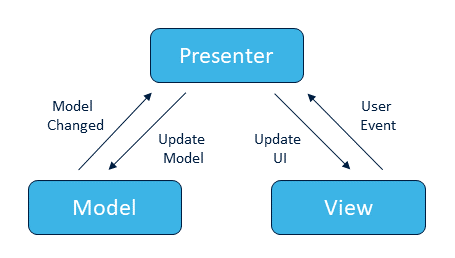
\includegraphics[width=16cm]{res/images/mvp.png}
	\caption{Model-View-Presenter}
	\label{fig:Model-View-Presenter}
\end{figure}

\subsubsection{Model}
Il Model è la parte dell'archittetura che ha il compito di gestire i dati e rappresenta il layer di persistenza dell'applicazione. La maggior parte delle operazioni e dei controlli vengono svolti al suo interno. Contiene anche i metodi che avviano le connessioni alle API ed interagiscono con esse eseguendo numerose funzionalità. Vi sono, ad esempio, i metodi che consentono la comunicazione con il backend.


\subsubsection{View}
La View ha la responsabilità di passare i dati al Presenter. Essa è implementata da:
\begin{itemize}
	\item Attività (Activity); \\
	\item Qualsiasi forma grafica con cui l'utente finale dell'applicazione andrà ad interagire. \\	
\end{itemize}

\subsubsection{Presenter}
Il Presenter funge da livello intermedio tra la View e il Model. Tutta la logica di presentazione appartiene ad esso ed è responsabile dell'interrogazione del modello e l'aggiornamento della vista, reagendo alle interazioni che compie l'utente nella UI. Un valore aggiunto è che il Presenter dipende dall'astrazione della View e non dalla sua concretizzazione, quindi non conosce la sua implementazione. Tutto ciò favorisce ad una più facile attività di test.

\subsubsection{Contract}
Il Contract può essere visto come un contratto nel quale vengono definiti tutti i metodi che verranno utilizzati dalla View, dal Presenter e dal Model. Quando si ha intenzione di scrivere una nuova funzionalità, è buona norma scrivere un Contract. Esso descrive la comunicazione tra View-Presenter e Model-Presenter, consentendo una progettazione più pulita e diminuire le dipendenze tra le componenti.
Il Contract è un'interfaccia e contiene le altre interfacce della View, Presenter e Model per garantire le varie comunicazioni.


\subsection{Diagramma dei package}
Vengono presentati di seguito i diagrammi UML dei package relativi all'applicazione.

\subsubsection{Visione Generale}
Il package principale dell'applicazione è nominato \textit{com.example.bc19mobile}.
Nel seguente diagramma UML vengono mostrate tutte le dipendenze che esistono tra i vari package.
\begin{figure}[H]
	\centering
	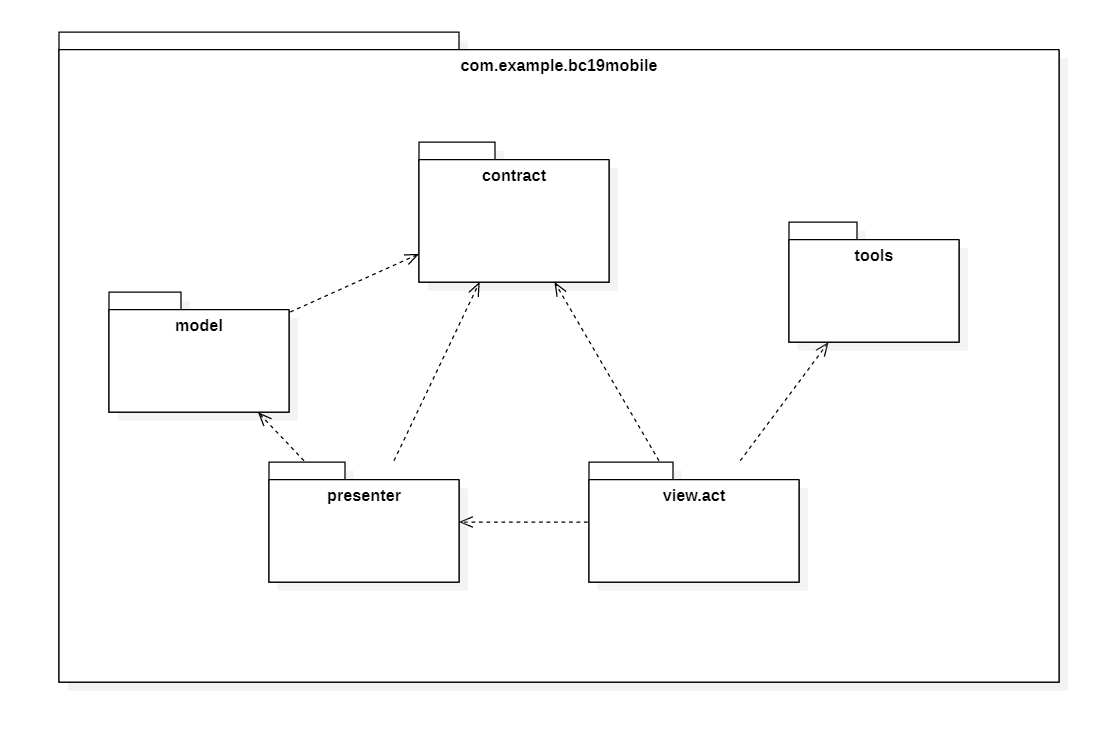
\includegraphics[width=16cm]{res/images/apputenti-packageGenerale.png}
	\caption{Visione generale dei package}
	\label{fig:Visione generale dei package}
\end{figure}

\subsubsection{Model}
Nel seguente package vengono raggruppati altri package contenenti tutte le classi utilizzate per la business logic. 
\begin{figure}[H]
	\centering
	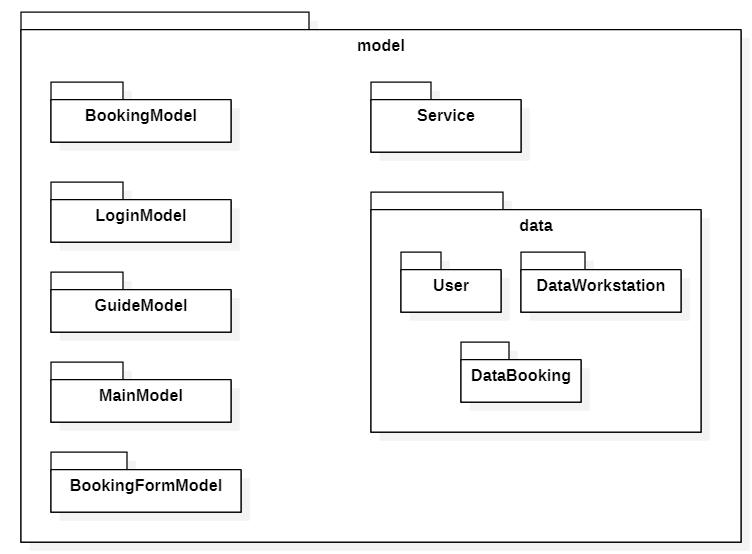
\includegraphics[width=16cm]{res/images/apputenti-packageModel.png}
	\caption{package-Model}
	\label{fig:package-Model}
\end{figure}


\subsubsection{View}
Nel seguente package vengono raggruppate tutte le classi dedicate alle funzionalità di user interface collegate con i loro rispettivi file XML che modificano la loro interpretazione grafica.
\begin{figure}[H]
	\centering
	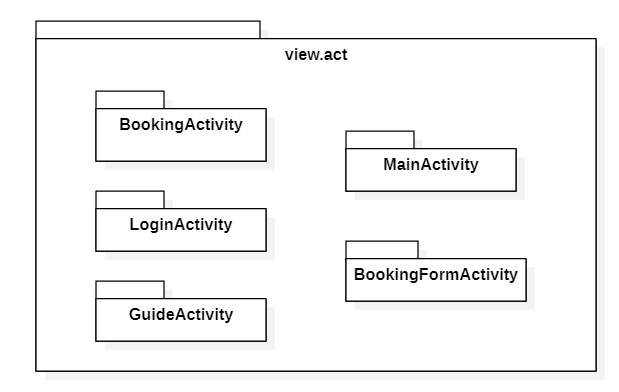
\includegraphics[width=16cm]{res/images/apputenti-packageView.png}
	\caption{package-View}
	\label{fig:package-View}
\end{figure}

\subsubsection{Presenter}
Nel seguente package vengono raggruppate tutte le classi dedicate alla comunicazione tra le altre due componenti dell'architettura.
\begin{figure}[H]
	\centering
	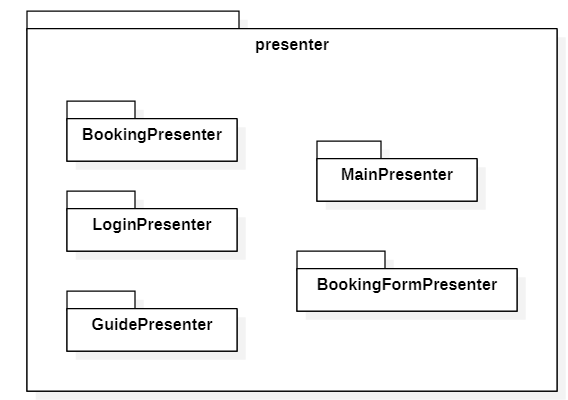
\includegraphics[width=16cm]{res/images/apputenti-packagePresenter.png}
	\caption{package-Presenter}
	\label{fig:package-Presenter}
\end{figure}

\subsubsection{Contract}
Nel seguente package vengono raggruppate tutte le interfacce Contract che servono per facilitare la comunicazione tra le varie componenti di MVP. Visto che a loro volta contengono altre interfacce possono essere rappresentate come dei "package".
\begin{figure}[H]
	\centering
	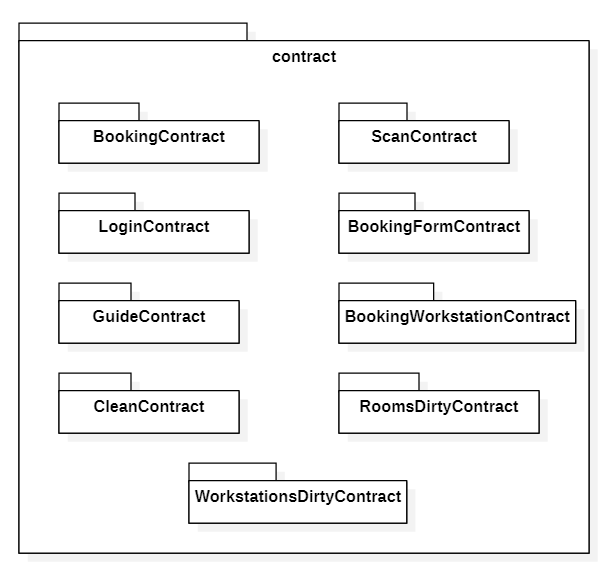
\includegraphics[width=16cm]{res/images/apputenti-packageContract.png}
	\caption{package-Contract}
	\label{fig:package-Contract}
\end{figure}

\subsubsection{Tool}
Nel seguente package vengono raggruppate tutte le classi ed interfacce dedicate alle funzionalità generiche che possono essere usate in base ai contesti per dare supporto alla vista.
\begin{figure}[H]
	\centering
	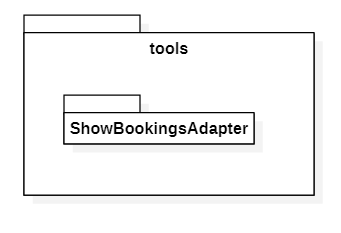
\includegraphics[width=16cm]{res/images/apputenti-packageTools.png}
	\caption{package-Tool}
	\label{fig:package-Tool}
\end{figure}

\subsection{Diagramma delle classi}
Vengono presentati di seguito i diagrammi UML delle classi relativi all'applicazione.

\subsubsection{Login}
\begin{figure}[H]
	\centering
	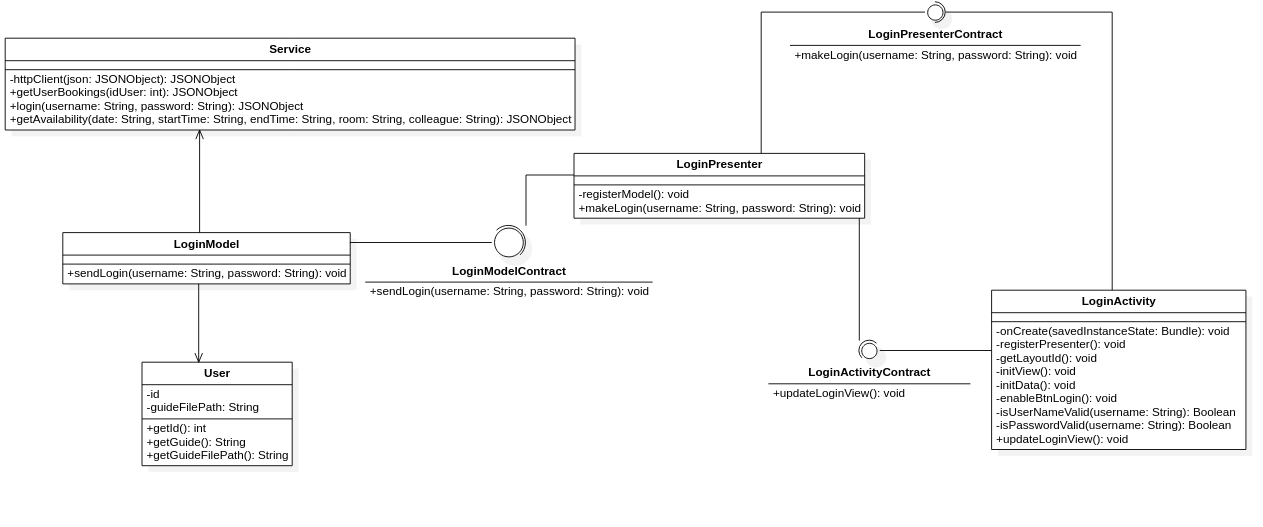
\includegraphics[width=16cm]{res/images/loginClass.png}
	\caption{Login-Diagramma delle classi}
	\label{fig:Login-Diagramma delle classi}
\end{figure}
La classe LoginActivity rappresenta la pagina dedicata all'autenticazione. L'utente inserisce username e password. Se registrato nel sistema l'utente potrà accedere all'applicazione altrimenti visualizzerà un messaggio d'errore.

La classe LoginActivity offre i seguenti metodi:
\begin{itemize}
	\item \textbf{onCreate(savedInstanceState:Bundle): void}: Si occupa della creazione della parte grafica visualizzata dall'utente; 
	\item \textbf{getLayoutId(): void}: associa il rispettivo file in formato xml alla View;
	\item \textbf{registerPresenter(): void}: associa il Presenter alla View;
	\item \textbf{initView(): void}: mappa l'Activity associandole le variabili: username, password, loginBtn, errore;
	\item \textbf{initData(): void}: definisce l'aggiornamento della vista secondo gli input dell'utente ;
	\item \textbf{enableBtnLogin(): void}: abilita il bottone di Login;
	\item \textbf{isUserNameValid(in username:String): Boolean}: verifica della conformità dell'username;
	\item \textbf{isPasswordValid(in username:String): Boolean}: verifica della conformità della password;
	\item \textbf{updateLoginView(): void}: aggiorna la vista dopo la verifica delle credenziali ;
\end{itemize}

La classe LoginPresenter offre i seguenti metodi:
\begin{itemize}
	\item \textbf{makeLogin(username: String, password: String): void}: Si occupa di richiedere al modello di effettuare il login; 
	\item \textbf{registerModel(): void}: associa il Model al Presenter.
\end{itemize}

La classe LoginModel offre i seguenti metodi:
\begin{itemize}
	\item \textbf{sendLogin(username: String, password: String): void}: Si occupa di richiedere al service di verificare le credenziali fornite dall'utente. 
\end{itemize}

La classe Service offre i seguenti metodi:
\begin{itemize}
	\item \textbf{login(in username:String, in password:String): JSONObject}: Si occupa di trasformare in un JSONObject username e password così poi da ottenere l'id dello user;
	\item \textbf{httpClient(json:JSONObject): JSONObject}: Viene fatta la richiesta al backend per verificare le credenziali fornite dall'utente.
	
\end{itemize}

\subsubsection{Main}
\begin{figure}[H]
	\centering
	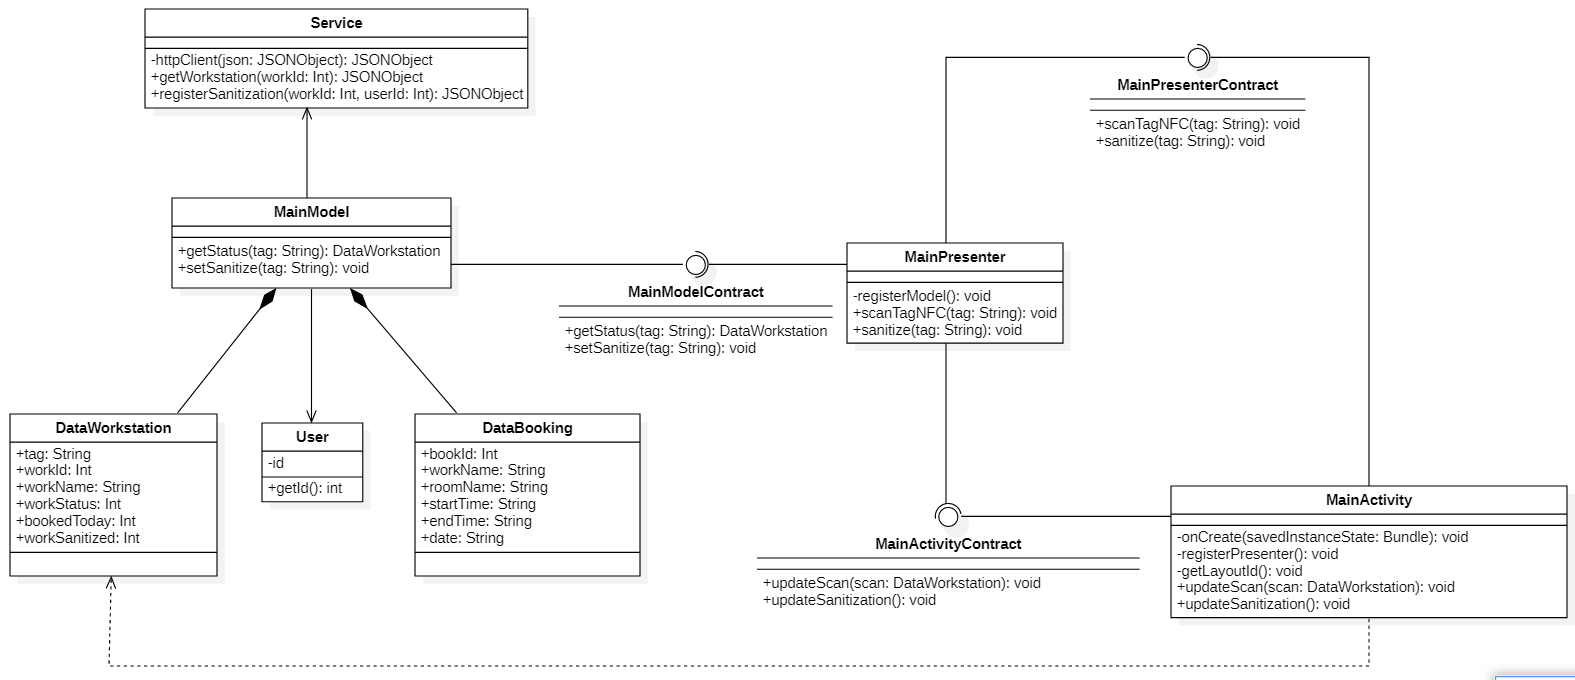
\includegraphics[width=16cm]{res/images/apputenti-MainClass.png}
	\caption{Main-Diagramma delle classi}
	\label{fig:Main-Diagramma delle classi}
\end{figure}
La classe MainActivity rappresenta la pagina principale dell'applicazione. Al suo interno è possibile eseguire varie operazioni premendo sul menù a tendina in alto a sinistra.
La funzione principale della classe MainActivity è la scansione dei tagNFC che ti permettono di visualizzare i seguenti campi:
\begin{itemize}
	\item wookId; 
	\item workName; 
	\item workStatus. 
\end{itemize}
In caso di prenotazioni, queste verranno mostrate.
Un'altra funzionalità di questa attività consiste nel premere sul bottone igienizzata una volta igienizzata la postazione così da cambiare stato e poter occupare la postazione se disponibile.

La classe MainActivity offre i seguenti metodi:
\begin{itemize}
	\item \textbf{onCreate(savedInstanceState:Bundle): void}: Si occupa della creazione della parte grafica visualizzata dall'utente; 
	\item \textbf{registerPresenter(): void}: associa il Presenter alla View; 
	\item \textbf{getLayoutId(): void}: associa il rispettivo file in formato xml alla View;
	\item \textbf{updateScan(scan:DataWorkstation): void}: Si occupa di far visualizzare le caratteristiche di una postazione dopo la scansione; 
	\item \textbf{updateSanitization(): void}: Si occupa di cambiare lo stato della postazione e disabilitare e nascondere il bottone per igienizzare. 
\end{itemize}

La classe MainPresenter offre i seguenti metodi:
\begin{itemize}
	\item \textbf{registerModel(): void}: associa il Model al Presenter; 
	\item \textbf{scanTagNFC(): void}: Si occupa di richiedere al modello le informazioni riguardanti la postazione, così poi da ritornarle alla vista; 
	\item \textbf{sanitize(): void}: Si occupa di richiedere al modello di igienizzare una postazione, così poi da ritornarlo alla vista. 
\end{itemize}

La classe MainModel offre i seguenti metodi:
\begin{itemize}
	\item \textbf{getStatus(): DataWorkstation}: Si occupa di richiedere al service le caratteristiche di una determinata postazione;
	\item \textbf{setSanitize(): void}: Si occupa di richiedere al service di igienizzare una determinata postazione.
\end{itemize}

La classe Service offre i seguenti metodi:
\begin{itemize}
	\item \textbf{registerSanitization(workId:Int, userId:Int): JSONObject}: Si occupa di trasformare in un JSONObject l'id dello user e l'id della postazione così poi da registrare l'igienizzazione;
	\item \textbf{getWorkstation(workId:Int): JSONObject}: Si occupa di trasformare in un JSONObject l'id della postazione così poi da ottenere le sue caratteristiche;
	\item \textbf{httpClient(json:JSONObject): JSONObject}: Viene fatta la richiesta al backend per ottenere le caratteristiche della postazione o per registrare l'igienizzazione.	
\end{itemize}

\subsubsection{Guide}
\begin{figure}[H]
	\centering
	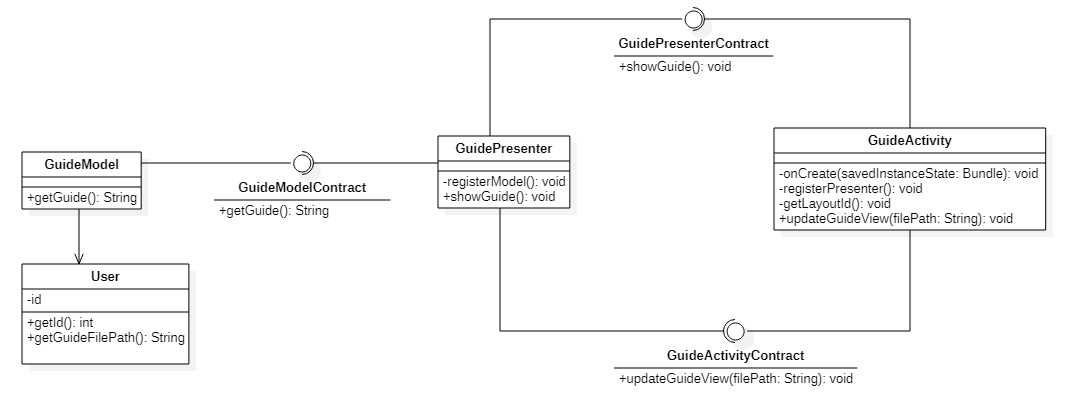
\includegraphics[width=16cm]{res/images/GuideActivity.png}
	\caption{GuideActivity-Diagramma delle classi}
	\label{fig:GuideActivity-Diagramma delle classi}
\end{figure}
La classe GuideActivity rappresenta la pagina dedicata alla visualizzazione della guida.
L'utente per visualizzare la guida deve premere sul menu a tendina del menù principale(MainActivity) e successivamente deve premere sulla voce "Guida" e verrà reindirizzato alla pagina dedicata.

In questa pagina verrà mostrata la guida dedicata all'utente. In base al suo identificativo con cui ha effettuato il login sarà possibile distinguerlo tra le due tipologie, dipendente e addetto alle pulizie, così da mostrare a ciascuno la guida corrispondente.

La classe GuideActivity offre i seguenti metodi:
\begin{itemize}
	\item \textbf{onCreate(savedInstanceState:Bundle): void}: Si occupa della creazione della parte grafica visualizzata dall'utente; 
	\item \textbf{getLayouId(): void}: associa il rispettivo file in formato xml alla View;
	\item \textbf{updateGuideView(in filePath:String): void}: Si occupa di far visualizzare il filePath sotto forma di stringa del percorso in cui viene salvato il documento della guida. 
\end{itemize}

La classe GuidePresenter offre i seguenti metodi:
\begin{itemize}
	\item \textbf{registerPresenter(): void}: associa il Presenter alla View; 
	\item \textbf{showGuide(): void}: Si occupa di richiedere al modello la guida, così poi da ritornarle alla vista. 
\end{itemize}

La classe GuideModel offre i seguenti metodi:
\begin{itemize}
	\item \textbf{registerModel(): void}: associa il Model al Presenter; 
	\item \textbf{getGuide(): String}: Si occupa di ottenere il filePath della guida di una determinata tipologia di utente, in base all'identificativo di quest'ultimo. 
\end{itemize}

\subsubsection{BookingForm}
\begin{figure}[H]
	\centering
	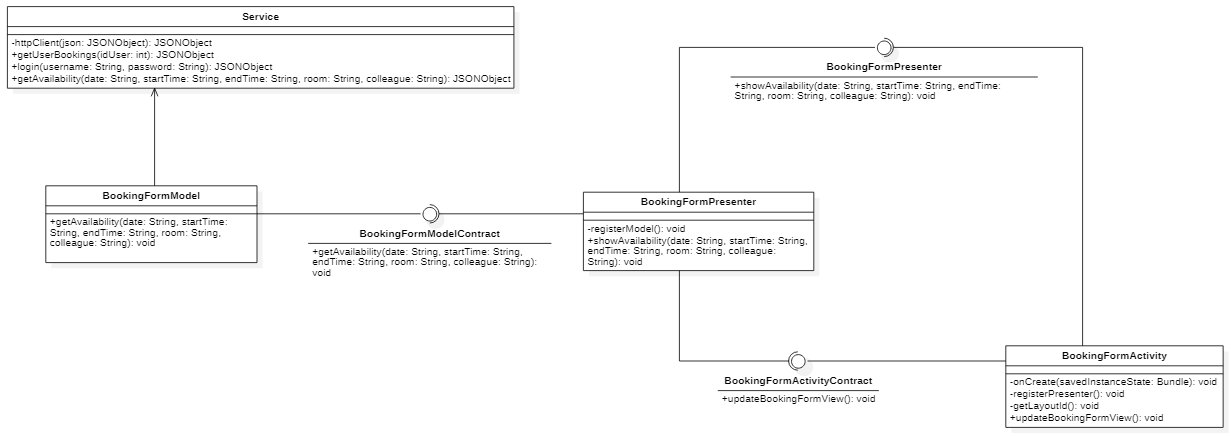
\includegraphics[width=16cm]{res/images/BookingForm.png}
	\caption{BookingForm-Diagramma delle classi}
	\label{fig:BookingForm-Diagramma delle classi}
\end{figure}
La classe BookingFormActivity rappresenta la pagina dedicata alla visualizzazione della ricerca di una postazione.
L'utente per visualizzare questa pagina deve premere sul menu a tendina del menù principale(MainActivity) e successivamente deve premere sulla voce "Prenota Postazione" e verrà reindirizzato alla pagina dedicata.

In questa pagina i campi da compilare sono: 
\begin{itemize}
	\item date; 
	\item startTime; 
	\item endTime; 
	\item room; 
	\item colleague. 
\end{itemize}

La classe BookingFormActivity offre i seguenti metodi:
\begin{itemize}
	\item \textbf{onCreate(savedInstanceState:Bundle): void}: Si occupa della creazione della parte grafica visualizzata dall'utente; 
	\item \textbf{getLayoutId(): void}: associa il rispettivo file in formato xml alla View;
	\item \textbf{updateBookingFormView(): void}: Si occupa di far visualizzare i campi da compilare tramite EditText nella pagina. Inoltre, per il campo data è possibile visualizzare una vista a calendario e per il campo ora una vista a orologio.
\end{itemize}

La classe BookingFormPresenter offre i seguenti metodi:
\begin{itemize}
	\item \textbf{registerPresenter(): void}: associa il Presenter alla View; 
	\item \textbf{showAvailability(in date:String, in startTime:String, in endTime:String, in room:String, in colleague:String): void}: Si occupa di richiedere al modello la disponibilità delle postazioni con i parametri dei campi inseriti, così poi da ritornarla alla vista. 
\end{itemize}

La classe BookingFormModel offre i seguenti metodi:
\begin{itemize}
	\item \textbf{registerModel(): void}: associa il Model al Presenter; 
	\item \textbf{getAvailability(in date:String, in startTime:String, in endTime:String, in room:String, in colleague:String): void}: Si occupa di richiedere al service la disponibilità delle postazioni con i parametri selezionati dall'utente. 
\end{itemize}

La classe Service offre i seguenti metodi:
\begin{itemize}
	\item \textbf{getUserBookings(idUser:int): JSONObject}: Si occupa di trasformare in un JSONObject l'id dello user;
	\item \textbf{httpClient(json:JSONObject): JSONObject}: Viene fatta la richiesta al backend per ottenere le postazioni disponibili;
	\item \textbf{login(in username:String, in password:String): JSONObject}: Si occupa di trasformare in un JSONObject lo username e password dello user;
	\item \textbf{getAvailability(in date:String, in startTime:String, in endTime:String, in room:String, in colleague:String): JSONObject}: Viene fatta la richiesta al backend per verificare la disponibilità delle postazioni filtrate in base ai parametri.
\end{itemize}


\subsubsection{Bookings}
\begin{figure}[H]
	\centering
	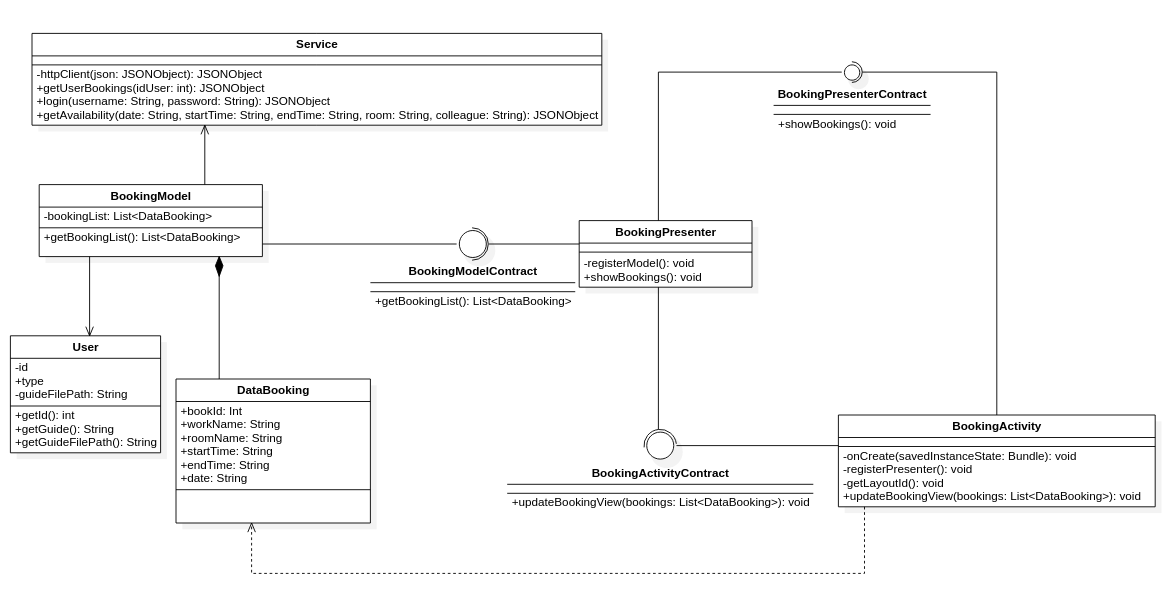
\includegraphics[width=16cm]{res/images/BookingsClass.png}
	\caption{Bookings-Diagramma delle classi}
	\label{fig:Bookings-Diagramma delle classi}
\end{figure}
La classe BookingActivity rappresenta la pagina dedicata alle prenotazioni effettuate da un utente. L'utente per visualizzare le prenotazioni deve premere sul menù a tendina del menù principale(MainActivity) e successivamente deve premere sulla voce "Visualizza Prenotazioni" e verrà reindirizzato alla pagina dedicata.

In questa pagina verranno mostrate in una lista tutte le prenotazioni effettuate dall'utente. Per ogni prenotazione i campi visualizzati sono: 
\begin{itemize}
	\item bookId; 
	\item workName; 
	\item roomName; 
	\item startTime; 
	\item endTime; 
	\item date. 
\end{itemize}
Nel caso non ci siano prenotazioni effettuate verrà mostrata una semplice stringa di testo con scritto: "Non ci sono prenotazioni effettuate".

La classe BookingActivity offre i seguenti metodi:
\begin{itemize}
	\item \textbf{onCreate(savedInstanceState:Bundle): void}: Si occupa della creazione della parte grafica visualizzata dall'utente; 
	\item \textbf{getLayoutId(): void}: associa il rispettivo file in formato xml alla View;
	\item \textbf{registerPresenter(): void}: associa il Presenter alla View;
	\item \textbf{updateBookingView(in bookings:List<DataBooking>): void}: Si occupa di far visualizzare le prenotazioni di un utente in una lista se ci sono, altrimenti deve far visualizzare la stringa "Non ci sono prenotazioni effettuate".
\end{itemize}

La classe BookingPresenter offre i seguenti metodi:
\begin{itemize}
	\item \textbf{showBookings(): void}: Si occupa di richiedere al modello la lista delle prenotazioni, così poi da restituirle alla vista; 
	\item \textbf{registerModel(): void}: associa il Model al Presenter.
\end{itemize}

La classe BookingModel offre i seguenti metodi:
\begin{itemize}
	\item \textbf{getBookingList(): List<DataBooking>}: Si occupa di richiedere al service le prenotazioni di un determinato utente. 
\end{itemize}

La classe Service offre i seguenti metodi:
\begin{itemize}
	\item \textbf{getUserBookings(idUser:int): JSONObject}: Si occupa di trasformare in un JSONObject l'id dello user così poi da ottenere la lista delle sue prenotazioni;
	\item \textbf{httpClient(json:JSONObject): JSONObject}: Viene fatta la richiesta al backend per ottenere la lista delle prenotazioni.
 
\end{itemize}

\subsection{Diagramma di sequenza}
Vengono presentati di seguito i diagrammi UML di sequenza relativi all'applicazione.

\subsubsection{Diagramma per il login}
\begin{figure}[H]
	\centering
	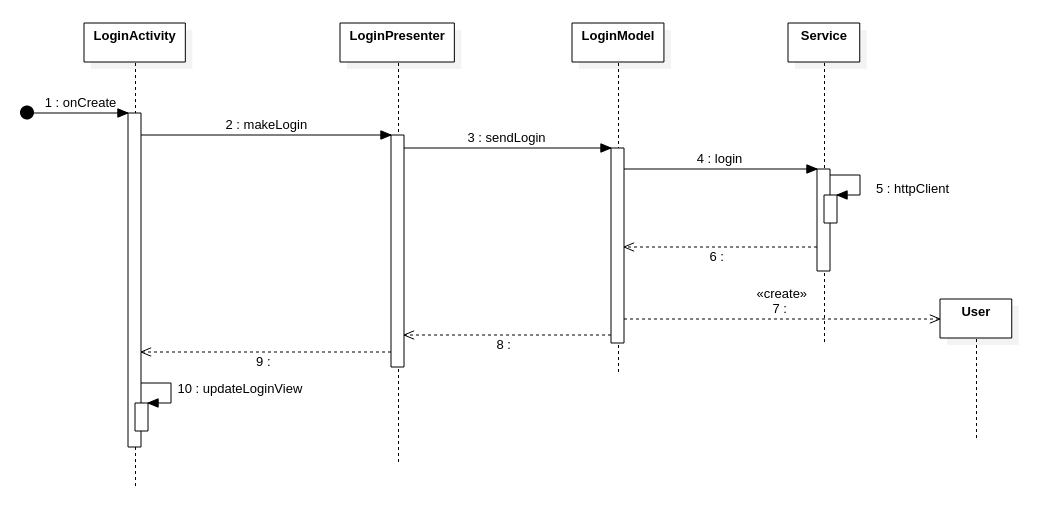
\includegraphics[width=16cm]{res/images/loginSeq.png}
	\caption{Login-Diagramma di sequenza}
	\label{fig:Login-Diagramma di sequenza}
\end{figure}
Questo diagramma di sequenza rappresenta la serie di azioni svolte dall'applicazione per autenticare un utente.
La sequenza inizia con la creazione della vista tramite il metodo \textit{onCreate}. Successivamente viene richiesto al Presenter di effettuare l'autenticazione tramite il metodo \textit{makeLogin} che a sua volta richiederà al Model di effettuare l'autenticazione attraverso il metodo \textit{sendLogin}.
Il Model chiama \textit{login} del Service tramite il quale genera il json con username e password. Ora il Service chiede di verificare al backend se esiste un utente associato a quelle credenziali tramite il metodo \textit{httpClient}.
Qualora l'utente esistesse viene creato un oggetto di classe User con l'id restituito da \textit{httpClient} e avvengono tutte le chiamate di ritorno.
Infine viene aggiornata la vista tramite il metodo \textit{updateLoginView}. 

\subsubsection{Diagramma per la visualizzazione delle prenotazioni di un utente}
\begin{figure}[H]
	\centering
	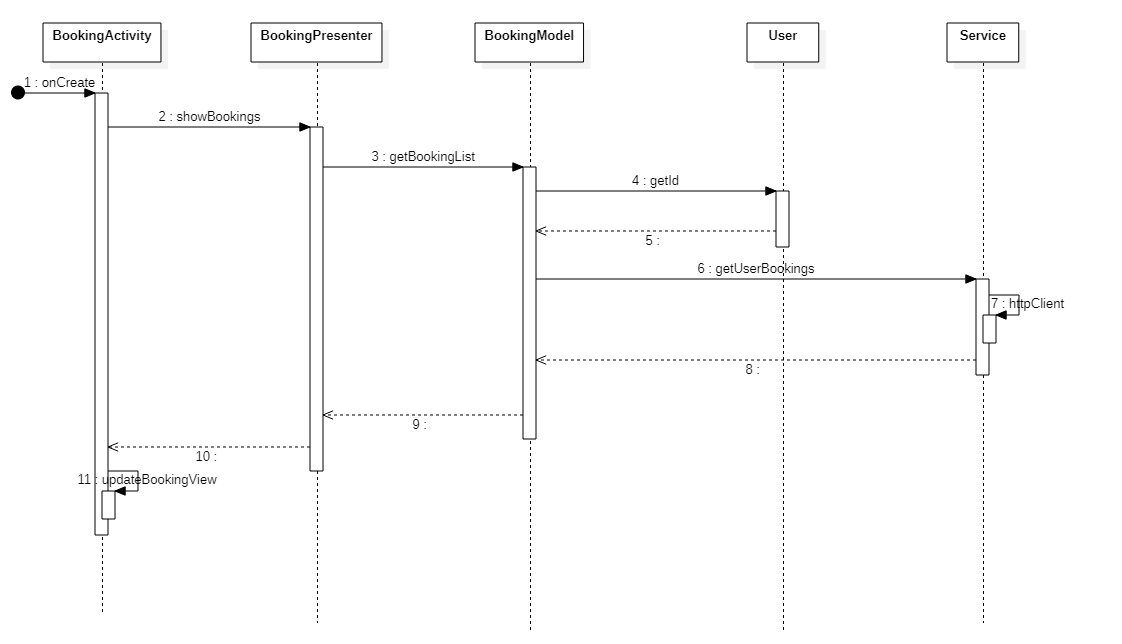
\includegraphics[width=16cm]{res/images/apputenti-showBookingsSeq.png}
	\caption{ShowBookings-Diagramma di sequenza}
	\label{fig:ShowBookings-Diagramma di sequenza}
\end{figure}
Questo diagramma di sequenza rappresenta la serie di azioni svolte dall'applicazione quando viene effettuata la richiesta di visualizzare le prenotazioni da un utente.
La sequenza inizia con la creazione della vista tramite il metodo \textit{onCreate}. Successivamente viene richiesto al Presenter di visualizzare le prenotazioni tramite il metodo \textit{showBookings} che a sua volta richiederà al Model la lista della prenotazioni attraverso il metodo \textit{getBookingList}.
Il Model per ottenere la lista delle prenotazioni farà prima una chiamata alla classe User con il metodo \textit{getId} per ottenere l'id dello user.
Il metodo successivo che deve usare è \textit{getUserBookings} con il quale genera il json con l'id dello user passandolo così al Service.
Il compito del Service è di ottenere la lista delle prenotazioni grazie al json trasmesso dal Model e quindi farà una chiamata con il metodo \textit{httpClient}.
In seguito verranno fatte tutte le chiamate di ritorno, ovvero verrà tornato al Model la lista delle prenotazioni che lo ritornerà al presenter che lo ritornerà a sua volta alla vista.
In conclusione per visualizzare la lista delle prenotazioni la vista chiamerà il metodo \textit{updateBookingView}. 

\subsubsection{Diagramma per ottenere le caratteristiche di una postazione}
\begin{figure}[H]
	\centering
	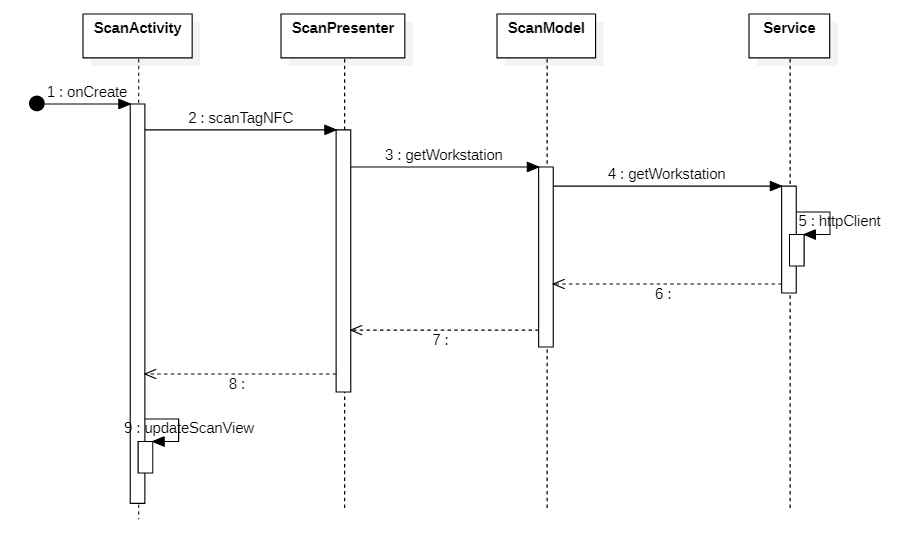
\includegraphics[width=16cm]{res/images/apputenti-mainScanSeq.png}
	\caption{Scan-Diagramma di sequenza}
	\label{fig:Scan-Diagramma di sequenza}
\end{figure}
Questo diagramma di sequenza rappresenta la serie di azioni svolte dall'applicazione quando viene effettuata scansionato un tag NFC da un utente.
La sequenza inizia con la creazione della vista tramite il metodo \textit{onCreate}.
Successivamente viene richiesto al Presenter di visualizzare le caratteristiche delle postazioni in seguito alla scansione del tag NFC tramite il metodo \textit{scanTagNFC} che a sua volta le richiederà al Model attraverso il metodo \textit{getStatus}.
Successivamente grazie a il metodo \textit{getWorkstation}, che genera un json con l'id della postazione, andrà a richiedere al Service tutte le caratteristiche. Per generare queste informazioni il Service userà il metodo \textit{httpClient}.
In seguito verranno fatte tutte le chiamate di ritorno, ovvero verrà tornato al Model le caratteristiche della postazione che lo ritornerà al presenter che lo ritornerà a sua volta alla vista.
In conclusione per visualizzare le informazioni di una postazione la vista chiamerà il metodo \textit{updateScan}.


\subsubsection{Diagramma per registrare l'igienizzazione di una postazione} 
\begin{figure}[H]
	\centering
	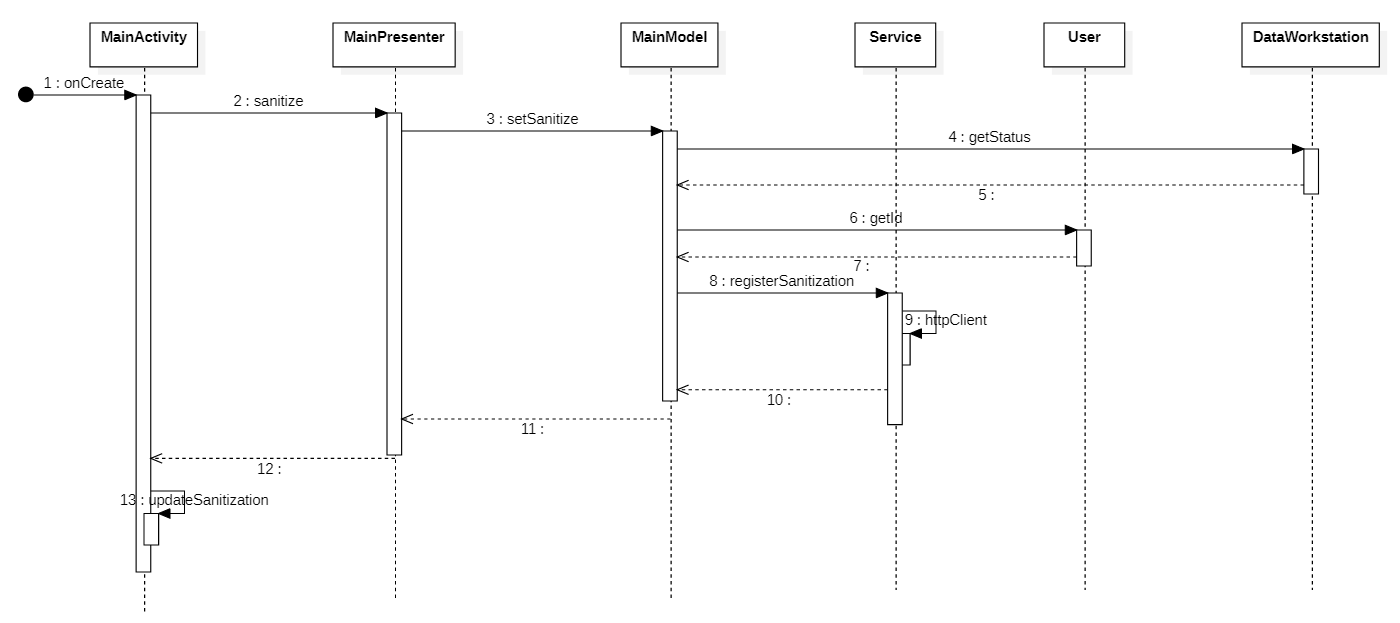
\includegraphics[width=16cm]{res/images/apputenti-mainSanitizeSeq.png}
	\caption{Sanitize-Diagramma di sequenza}
	\label{fig:Sanitize-Diagramma di sequenza}
\end{figure}
Questo diagramma di sequenza rappresenta la serie di azioni svolte dall'applicazione quando viene premuto da un utente il bottone per rendere una postazione igienizzata.
La sequenza inizia con la creazione della vista tramite il metodo \textit{onCreate}.
Successivamente viene richiesto al Presenter di registrare l'igienizzazione della postazione da parte di un utente tramite il metodo \textit{sanitize} che a sua volta lo richiederà al Model attraverso il metodo \textit{setSanitize}.
Il Model per ottenere igienizzare una postazione farà prima una chiamata alla classe User con il metodo \textit{getId} per ottenere l'id dello user.
Successivamente grazie a il metodo \textit{registerSanitization}, che genera un json con l'id della postazione e l'id dell'utente, andrà a richiedere al Service di registrarla. Per registrarla il Service userà il metodo \textit{httpClient}.
In seguito verranno fatte tutte le chiamate di ritorno, ovvero verrà tornato al Model il risultato dell'operazione che lo ritornerà al presenter che lo ritornerà a sua volta alla vista.
In conclusione per visualizzare le nuove informazioni sulla postazione la vista chiamerà il metodo \textit{updateSanitization}.

